% Activate the following line by filling in the right side. If for example the name of the root file is Main.tex, write
% "...root = Main.tex" if the chapter file is in the same directory, and "...root = ../Main.tex" if the chapter is in a subdirectory.
 
%!TEX root =  ../Thesis.tex

\chapter[Signal Kinematics]{Signal Kinematics}
 
\section{Signal Jet Kinematics}

\section{Signal Jet Combinatorics}

\section{Mass Resolution}
Once the trigger and all the analysis cuts have been applied, we take the leading 2 jets in the event (which are also the leading 2 $b$-tagged jets, since we place a cut requiring that the leading 2 jets in the event be $b$-tagged) and reconstruct their combined invariant mass--if they came from a decaying particle, the reconstructed mass should be the mass of the parent particle.  On the other hand, if the leading 2 jets come from continuum QCD processes, there should be no resonance present, so we look for the presence of a resonance peak on top of a decaying power-law background.

The sensitivity of this analysis depends on the signal cross section and efficiency, the background cross section and efficiency, but also the signal resolution.  The broader the signal mass peak, the more difficult it is to distinguish from the background.  

Unfortunately, the mass resolution significantly degrades as a $m_A$ grows.  Some of this is due to the inherent width growing as $m_A$ grows, as can be seen in Table~\ref{tab:sig_mc_parameters}.  

\subsection{Mass Resolution Improvement after Requiring that Leading Two Jets be $b$-Tagged}
The mass resolution also improves when we require that the leading two jets in the event be b-tagged;
 the plots in Figure 39 and Figure 40 show the ect on the invariant mass distribution.
 In order to quantify the mass resolution ect, we define the “left” and “right” shoulders of the mbb
 distribution, which are respectively the portion of the mbb distribution that are below and above the peak.
 go into further detail on the signal shape in Section 6.2; but in Table~\ref{tab:signal_mass_RMS_compare} the RMS of especially the left
 shoulder before and after requiring b-tags on the leading 2 jets quantitatively shows the mass resolution
 improvement.



%----------------------------------------------
\begin{table}
\centering
\caption{The RMS of the mass distribution in the left and right shoulders of the peak,
    as explained in the text.  The left shoulder is dominated by radiation off the Higgs
    and/or the Higgs daughter jets in addition to combinatorial mis-reconstructions,
    leading to a larger RMS than the right shoulder, which
    is dominated by combinatorics only.\label{tab:signal_mass_RMS_compare}   }
  \begin{tabular}{ccccc}
     \hline \hline
     generated mass (GeV) & \multicolumn{2}{c}{require $b$-tags on leading 2 jets (GeV)} & \multicolumn{2}{c}{no $b$-tag required on leading 2 jets (GeV)}  \\
        & left & right & left & right \\ \hline
     250 & 13.5 & 89.2 & 36.7 & 87.7 \\
     280 & 19.2 & 68.8 & 27.5 & 71.4 \\
     310 & 19.2 & 58.3 & 31.8 & 58.1 \\
     350 & 28.3 & 34.5 & 33.9 & 36.2 \\
     400 & 33.4 & 26.1 & 45.1 & 26.5 \\
     450 & 39.5 & 25.7 & 62.2 & 25.9 \\
     500 & 48.6 & 29.3 & 81.1 & 29.8 \\
     550 & 54.9 & 31.1 & 93.1 & 33.3 \\
     600 & 73.0 & 26.0 & 117.6 & 30.5 \\
     650 & 75.4 & 31.7 & 130.8 & 31.8 \\
     700 & 75.7 & 40.3 & 143.4 & 40.7 \\
     800 & 100.9 & 36.2 & 177.4 & 36.3 \\
     \hline     \end{tabular}
\end{table}
%----------------------------------------------


%----------------------------------------------
\begin{figure}
    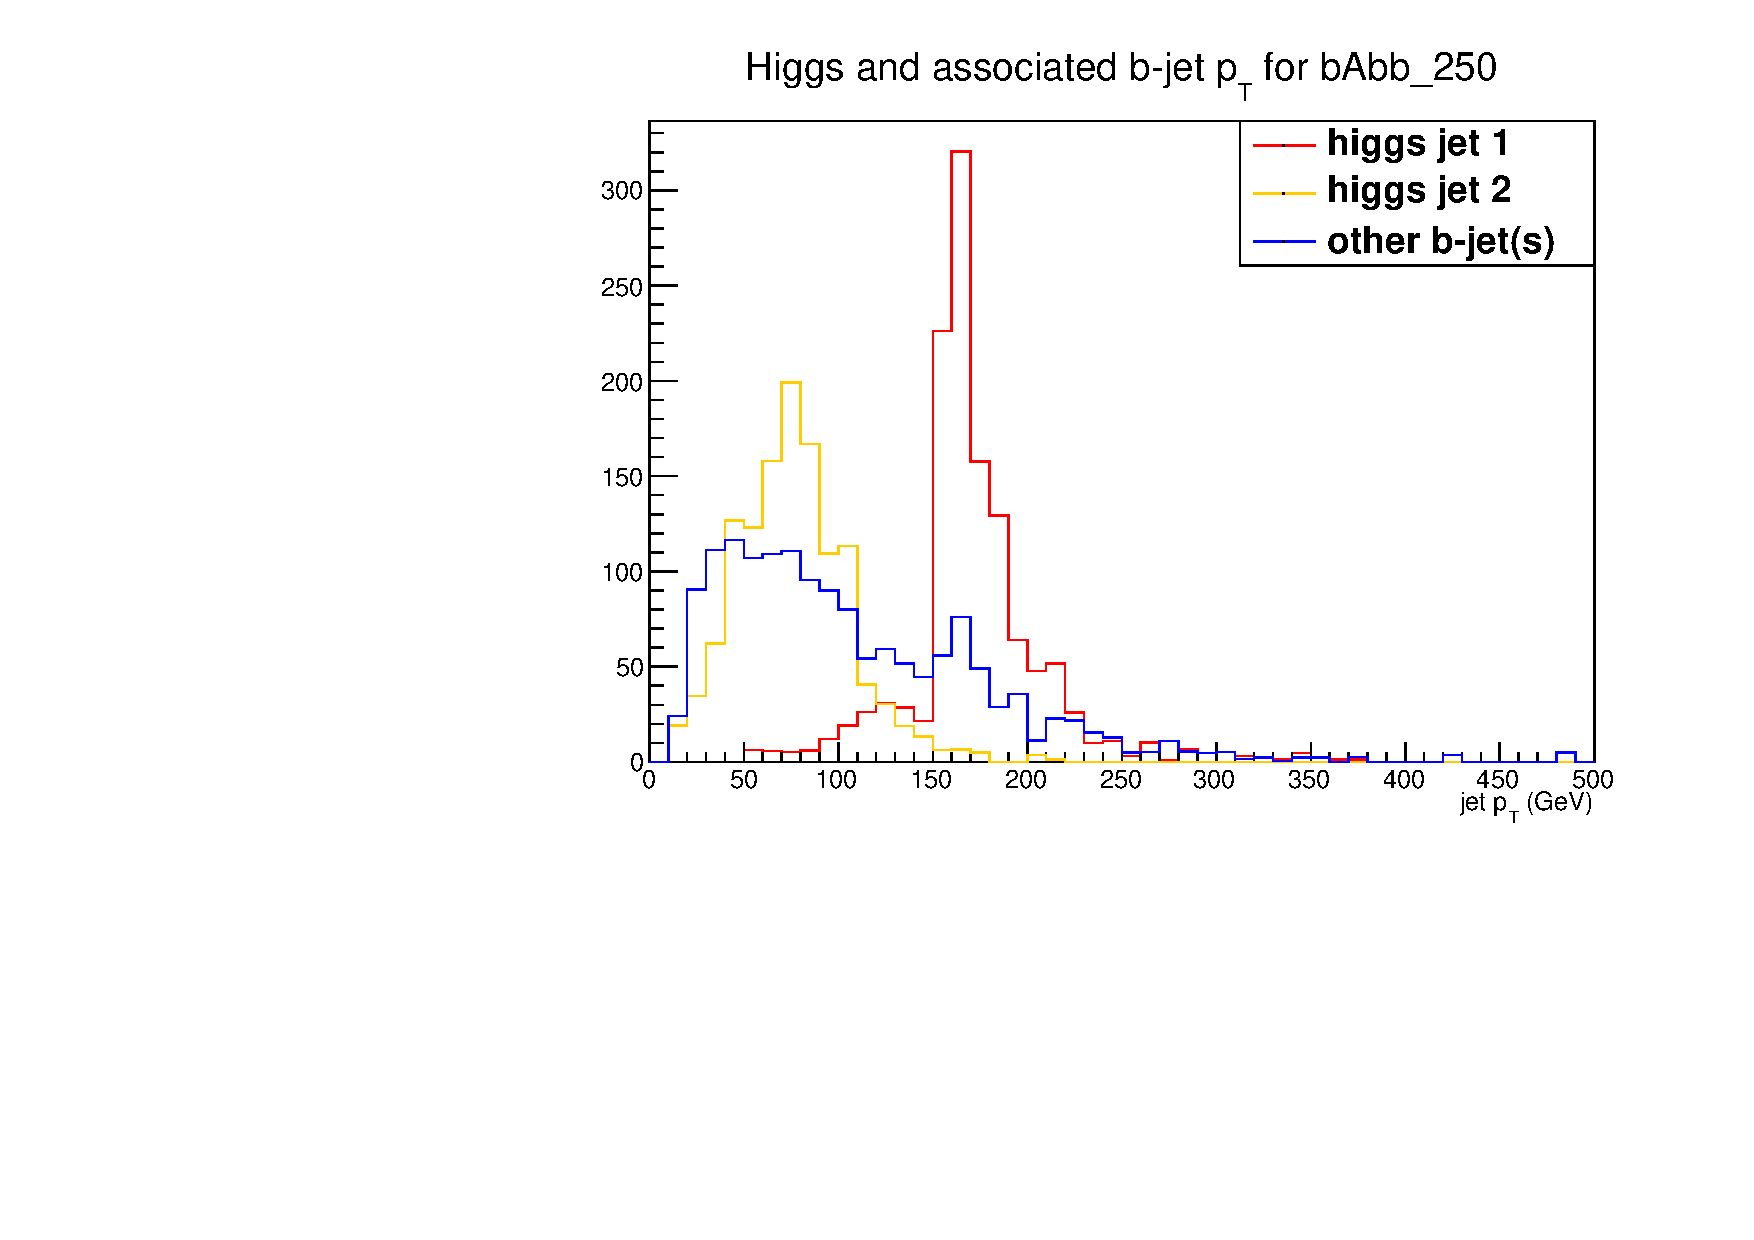
\includegraphics[width=0.33\textwidth]{/Users/caitlinmalone/Documents/Thesis/SignalKin/jet_pt_compare_bAbb_250.pdf}
    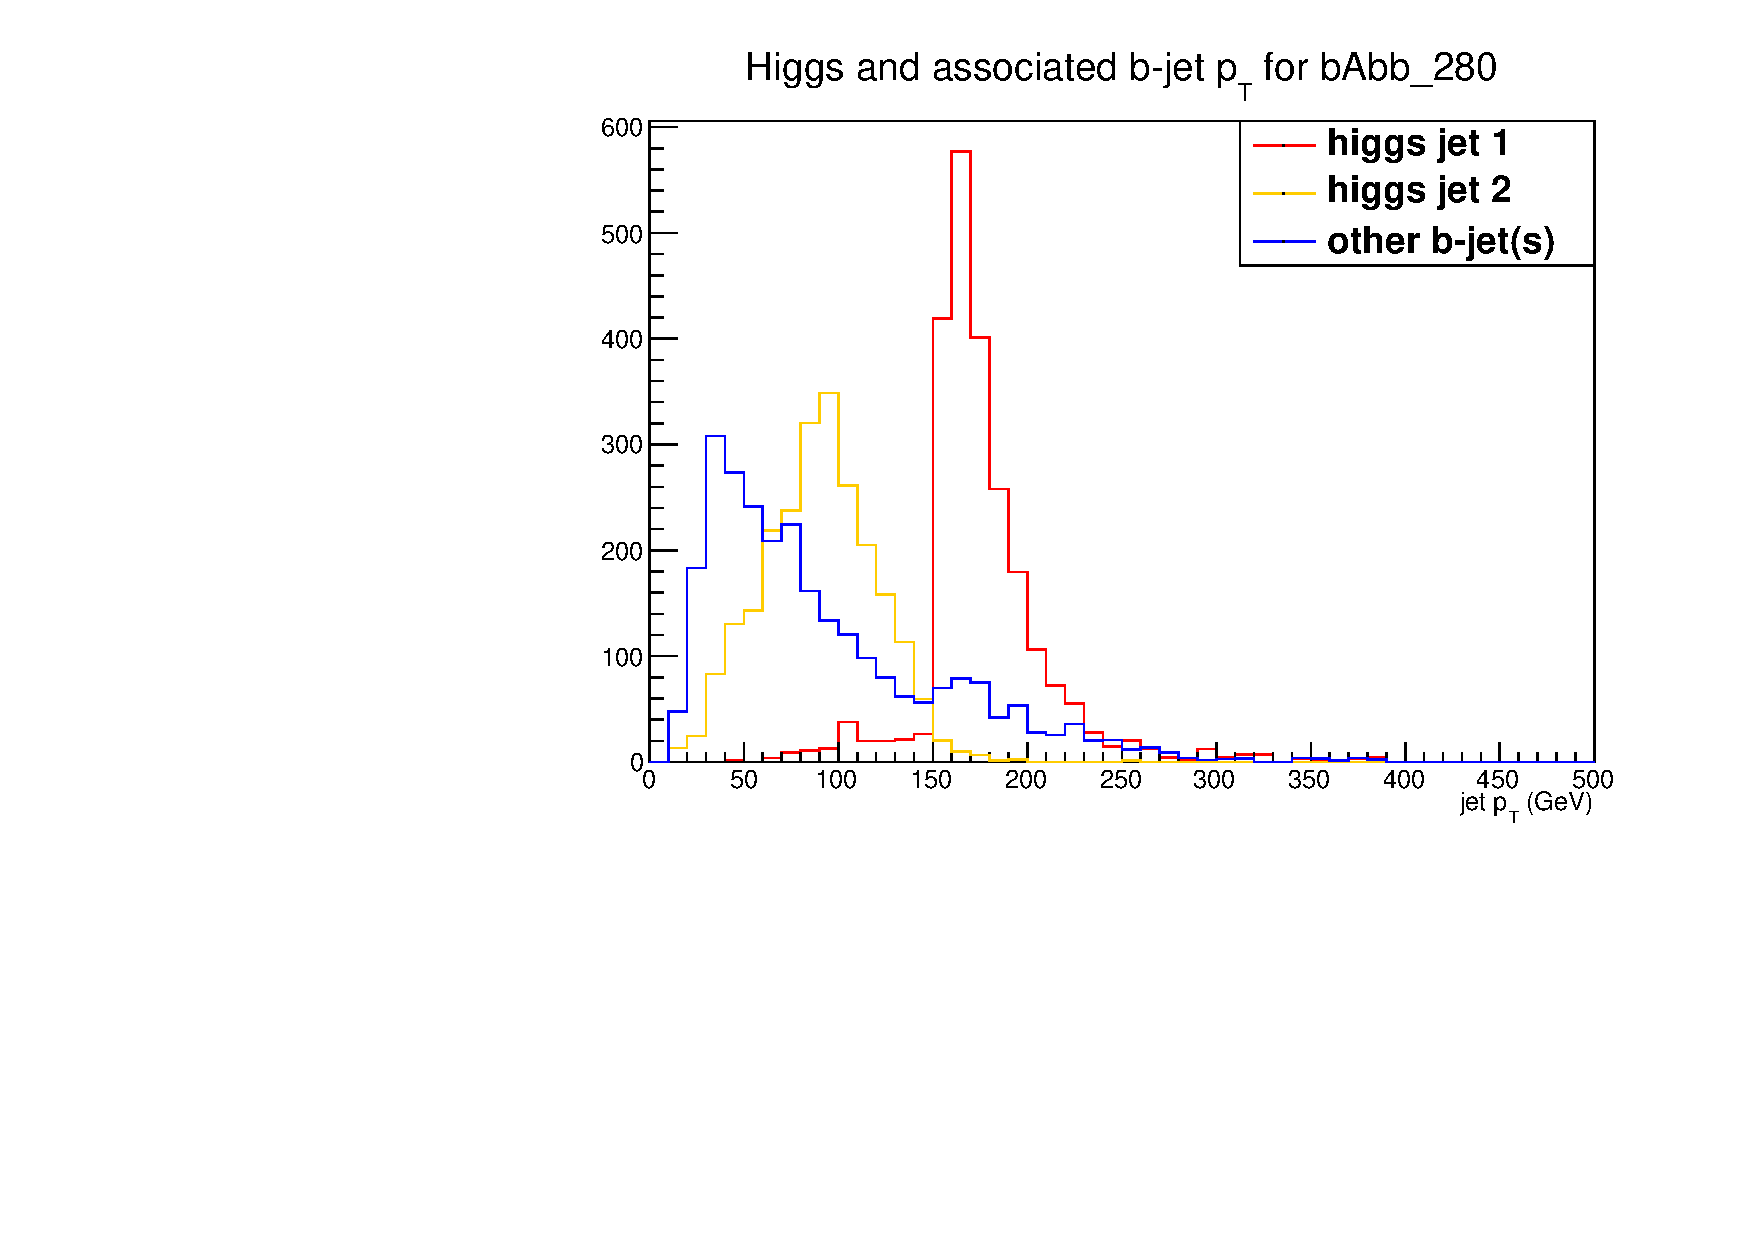
\includegraphics[width=0.33\textwidth]{/Users/caitlinmalone/Documents/Thesis/SignalKin/jet_pt_compare_bAbb_280.pdf}
    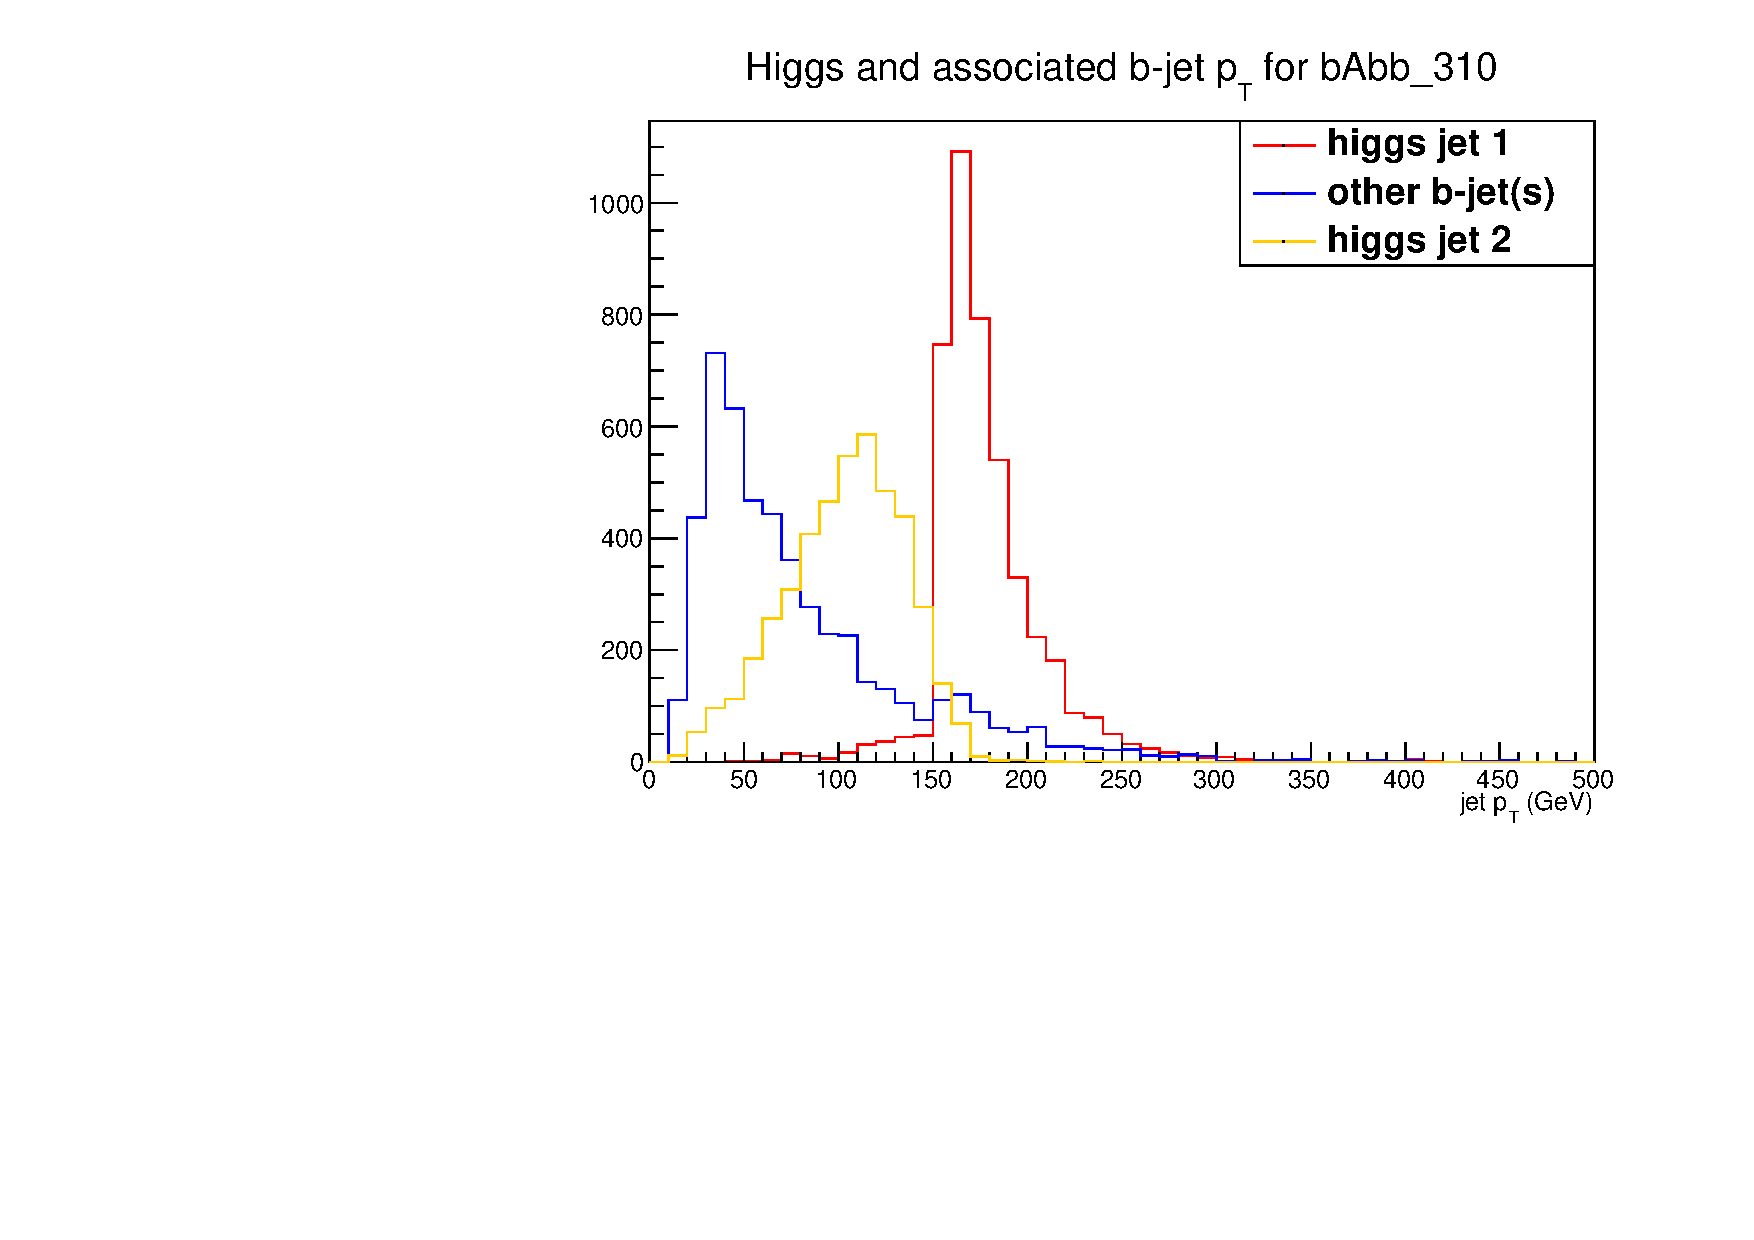
\includegraphics[width=0.33\textwidth]{/Users/caitlinmalone/Documents/Thesis/SignalKin/jet_pt_compare_bAbb_310.pdf}
%    \newline
    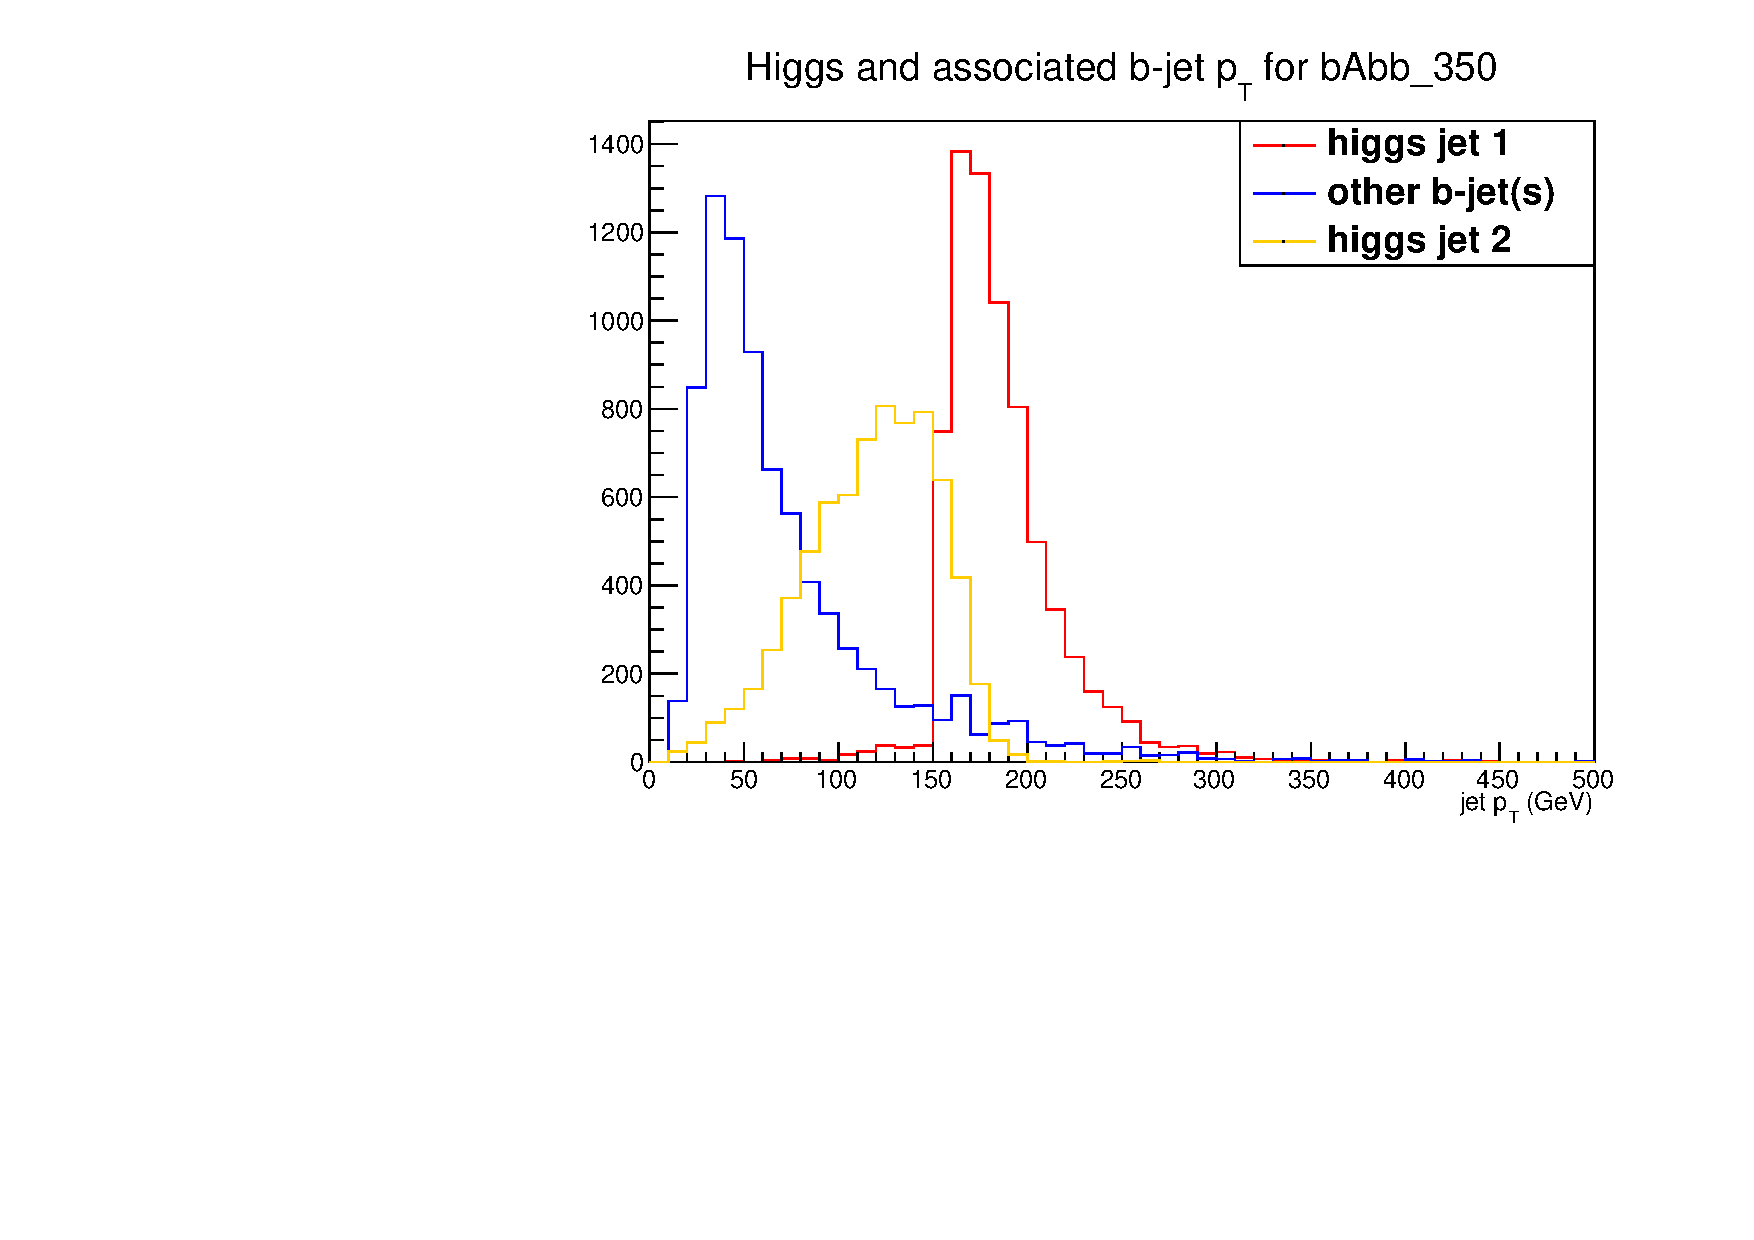
\includegraphics[width=0.33\textwidth]{/Users/caitlinmalone/Documents/Thesis/SignalKin/jet_pt_compare_bAbb_350.pdf}
    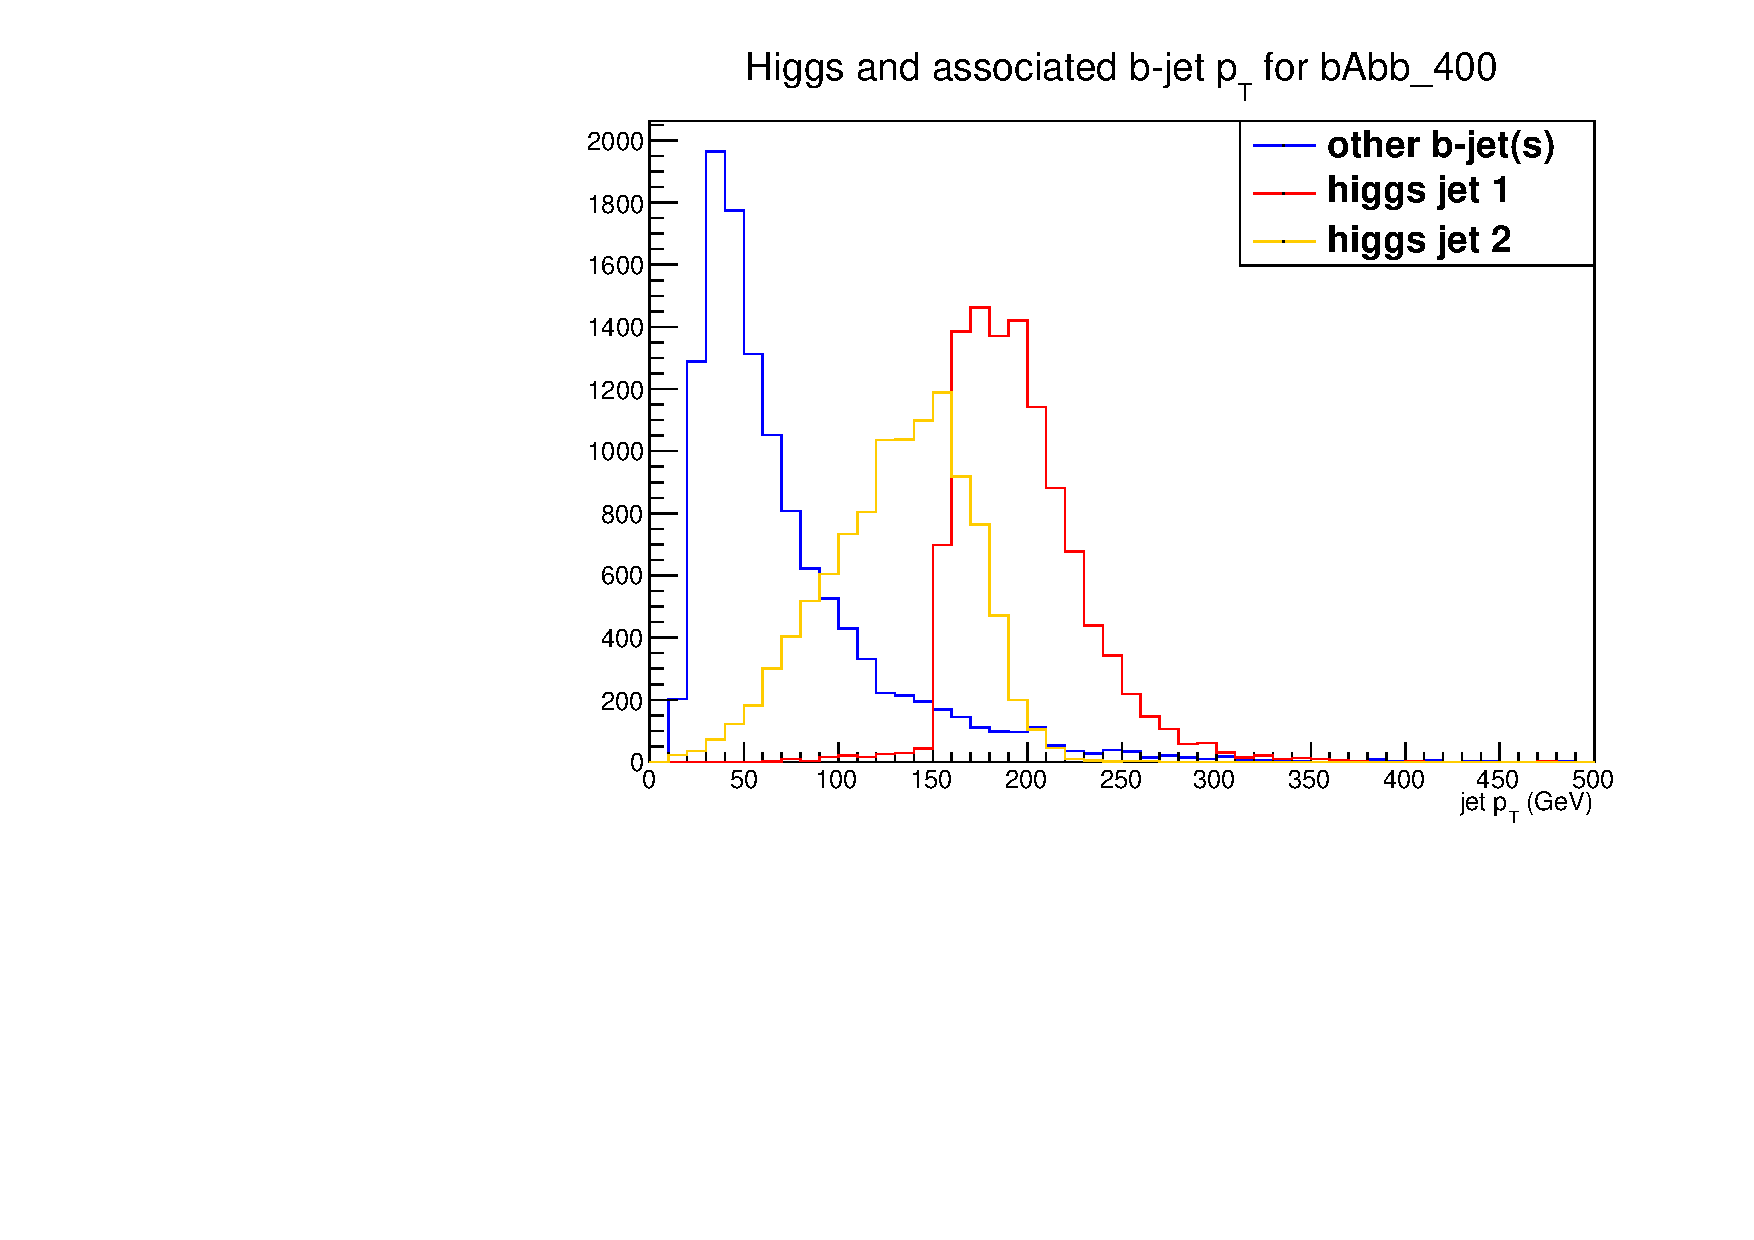
\includegraphics[width=0.33\textwidth]{/Users/caitlinmalone/Documents/Thesis/SignalKin/jet_pt_compare_bAbb_400.pdf}
    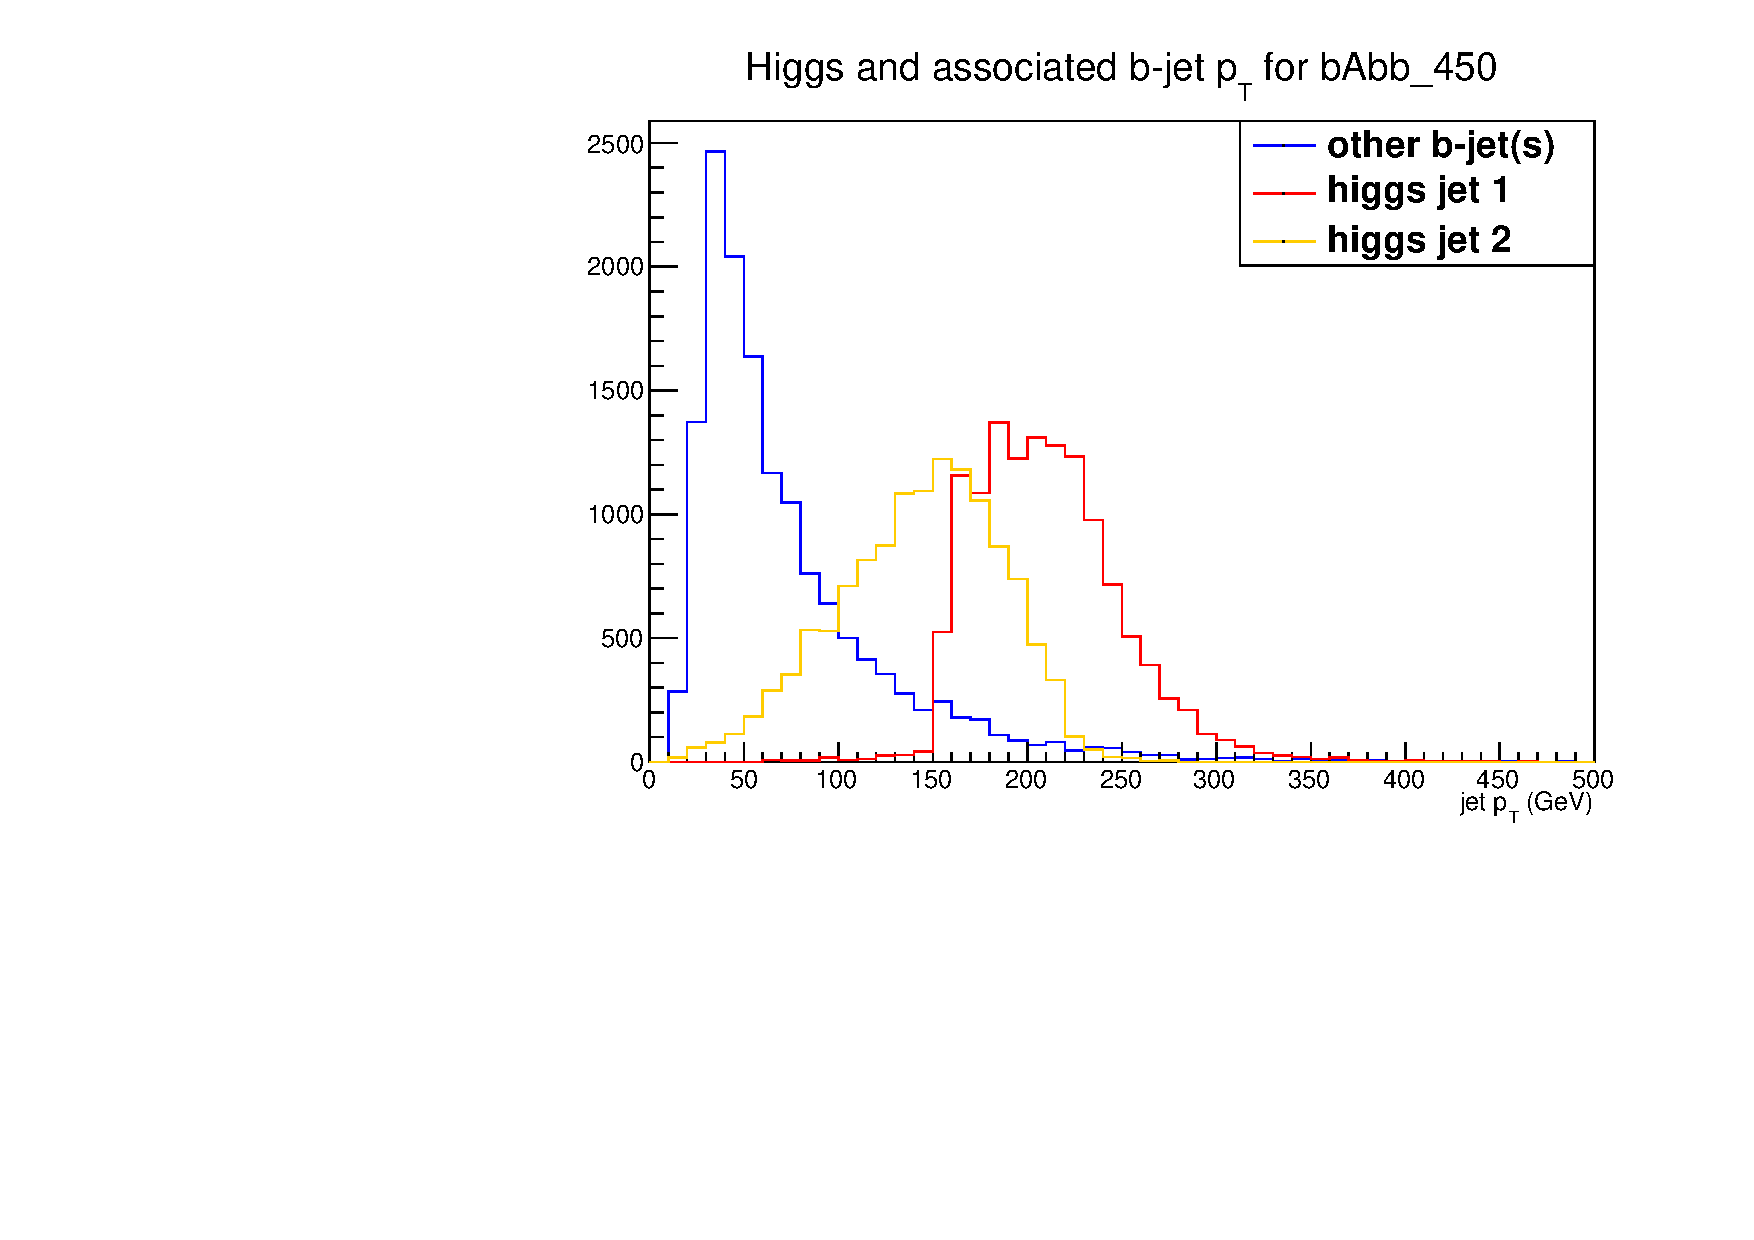
\includegraphics[width=0.33\textwidth]{/Users/caitlinmalone/Documents/Thesis/SignalKin/jet_pt_compare_bAbb_450.pdf}
%    \newline
    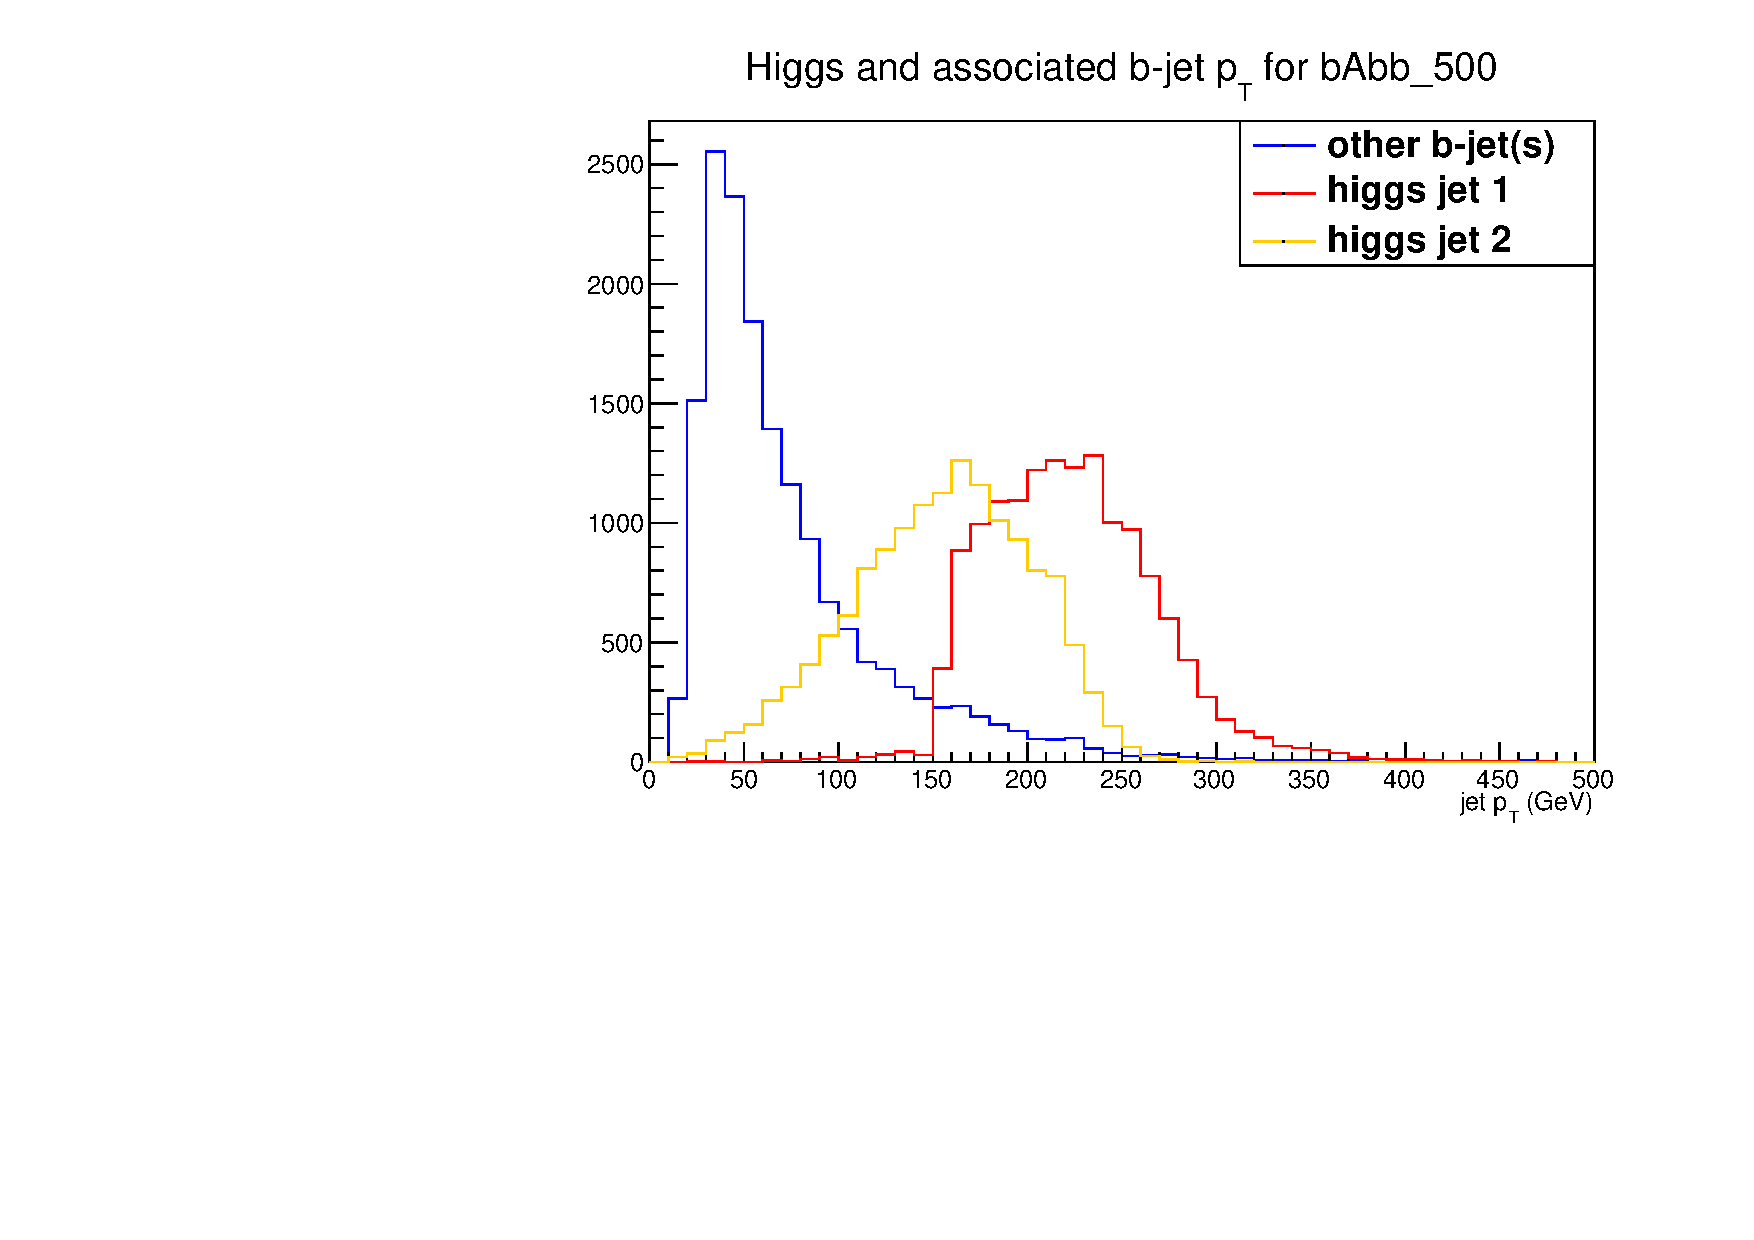
\includegraphics[width=0.33\textwidth]{/Users/caitlinmalone/Documents/Thesis/SignalKin/jet_pt_compare_bAbb_500.pdf}
    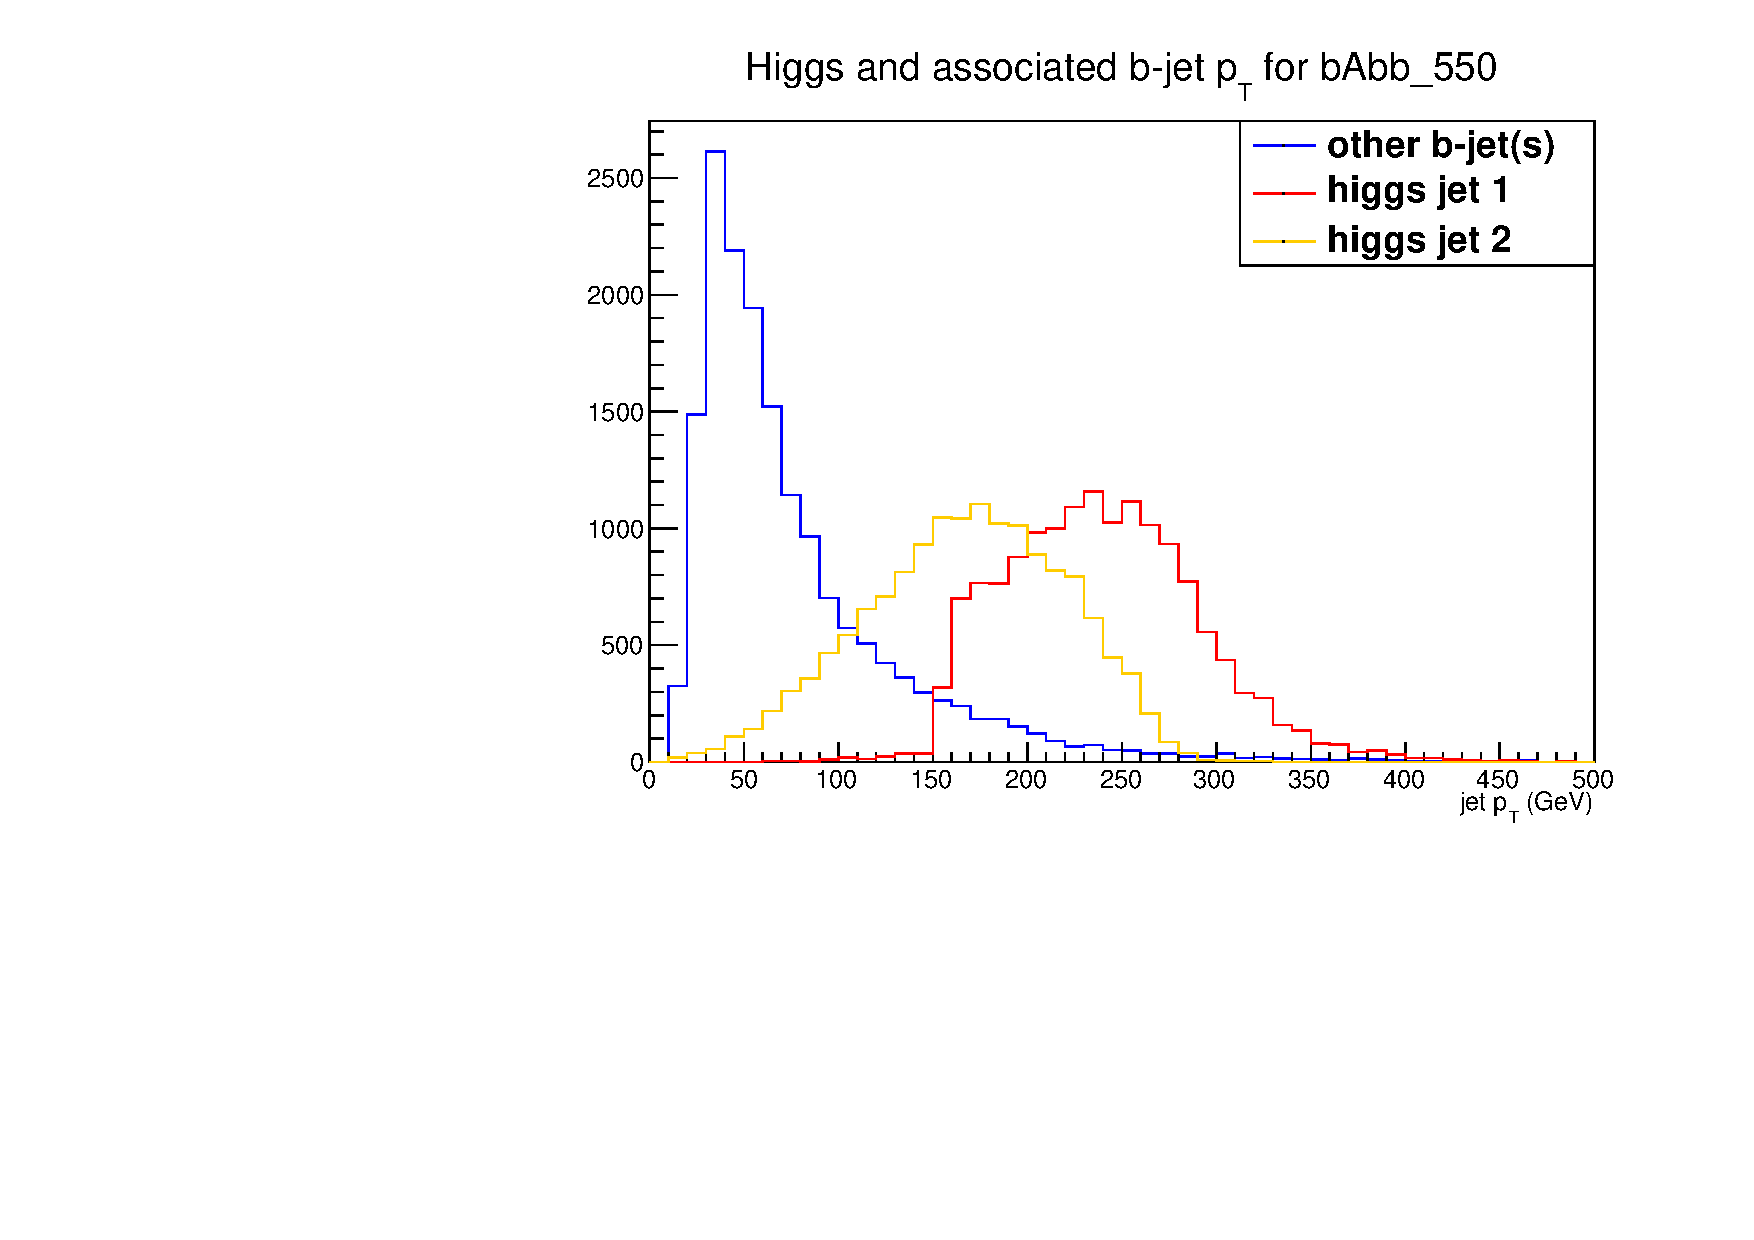
\includegraphics[width=0.33\textwidth]{/Users/caitlinmalone/Documents/Thesis/SignalKin/jet_pt_compare_bAbb_550.pdf}
    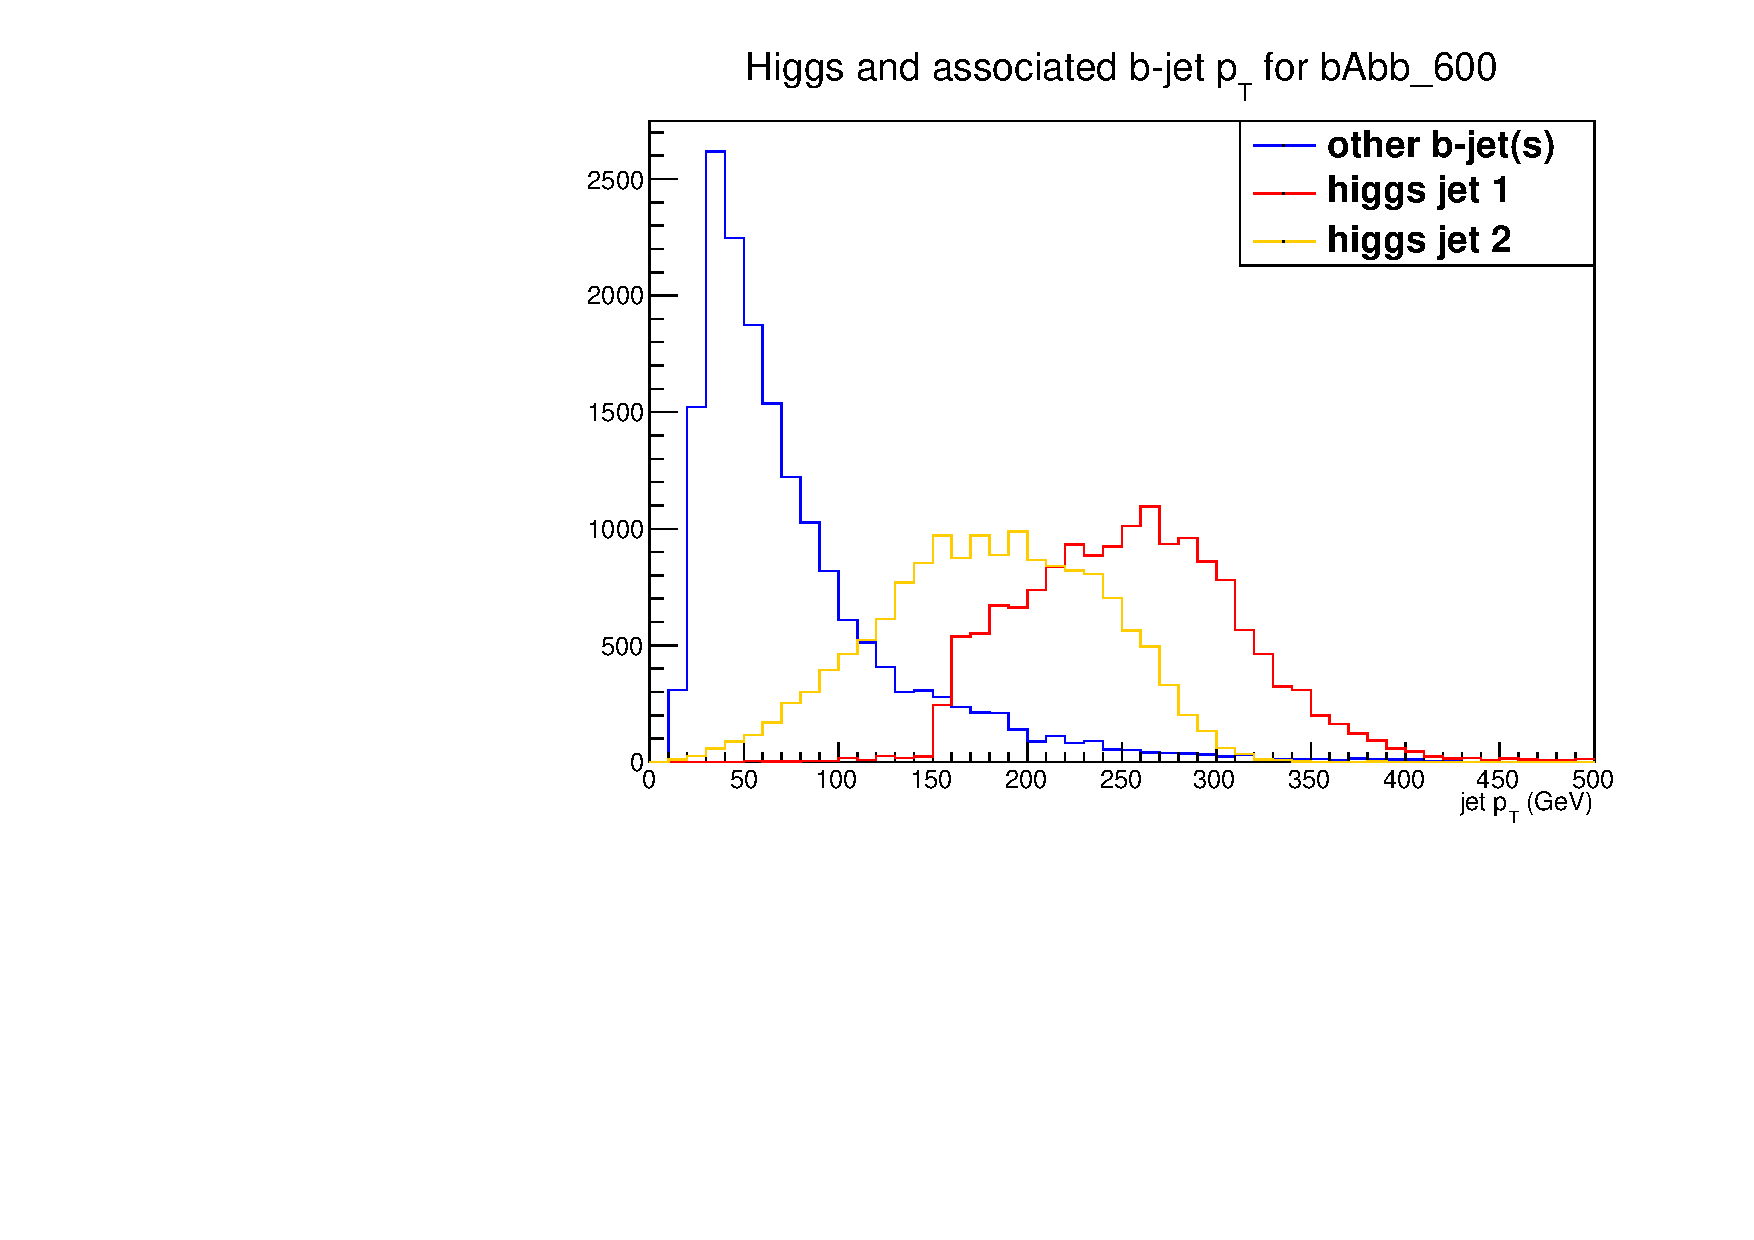
\includegraphics[width=0.33\textwidth]{/Users/caitlinmalone/Documents/Thesis/SignalKin/jet_pt_compare_bAbb_600.pdf}
%    \newline
    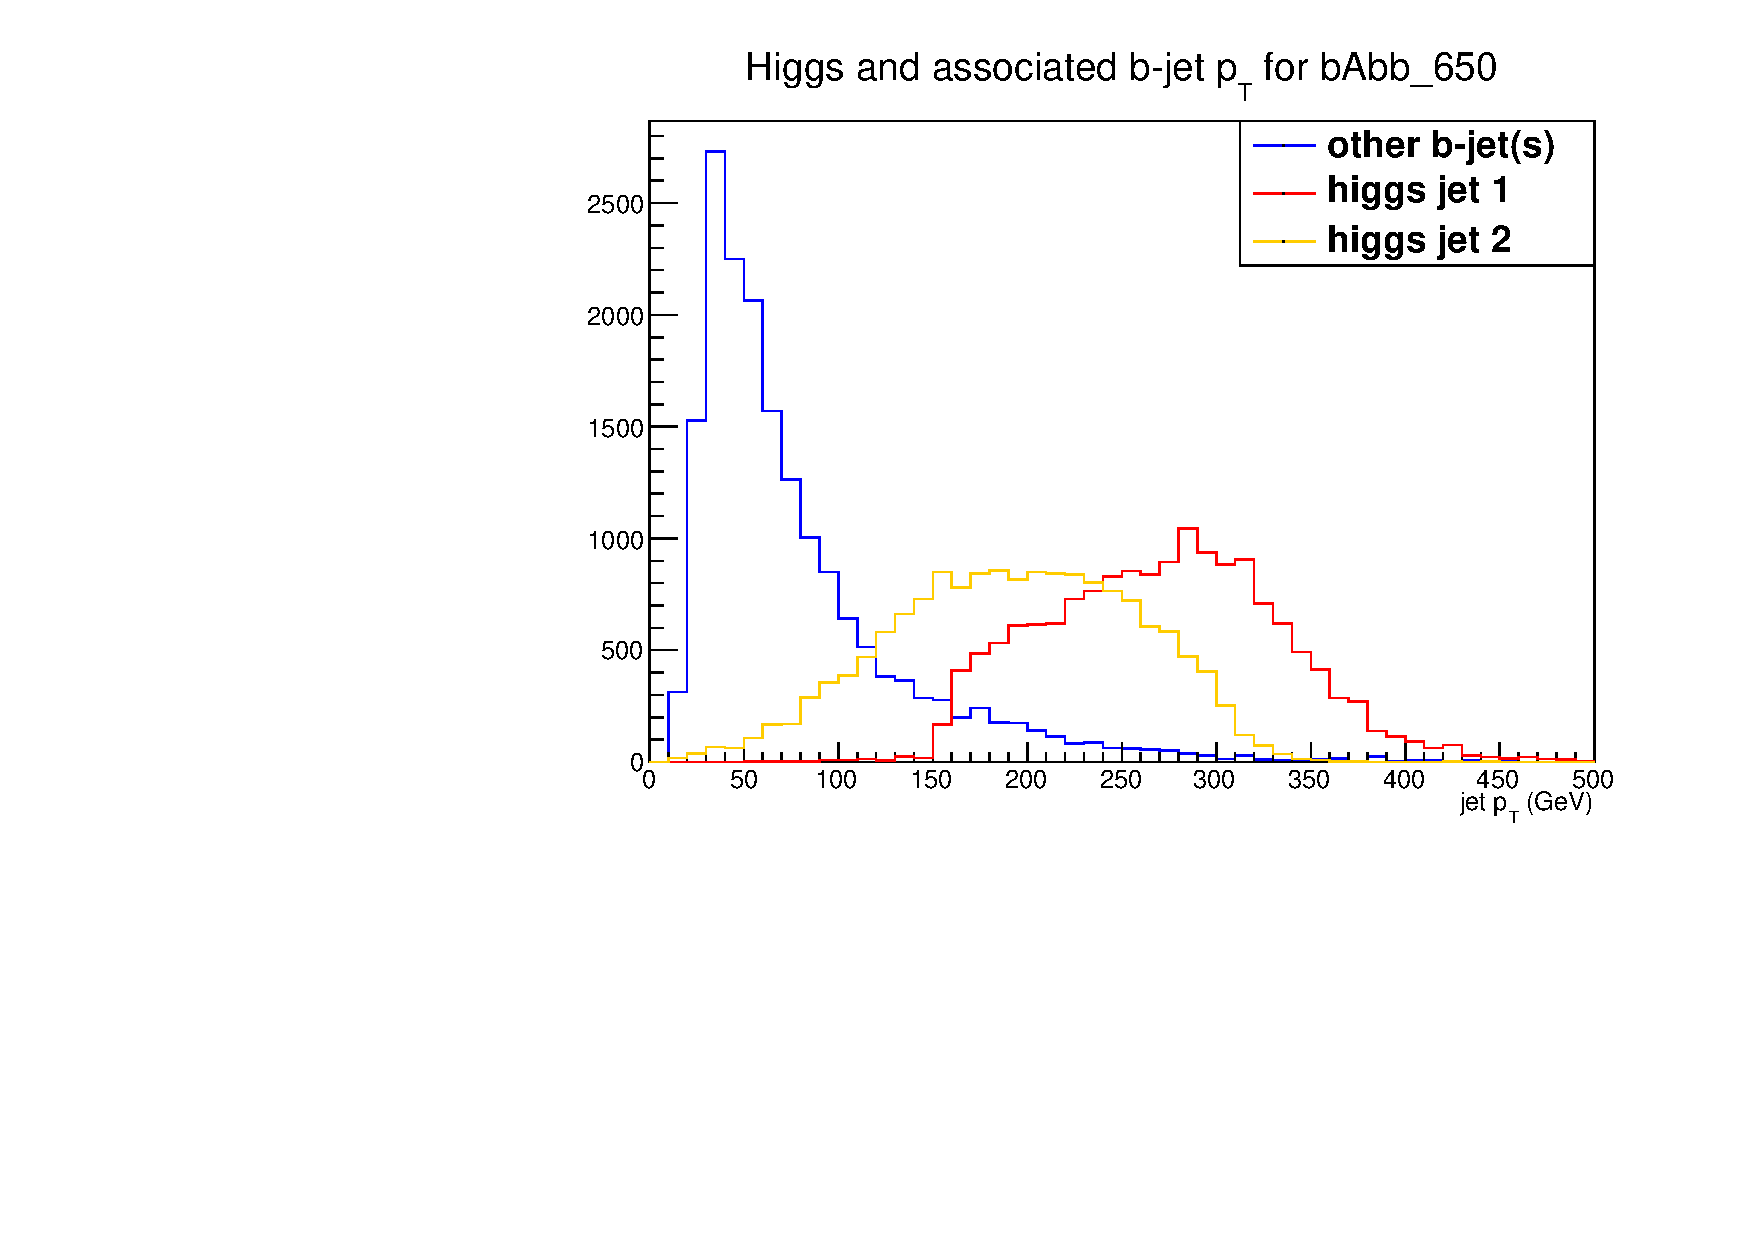
\includegraphics[width=0.33\textwidth]{/Users/caitlinmalone/Documents/Thesis/SignalKin/jet_pt_compare_bAbb_650.pdf}
    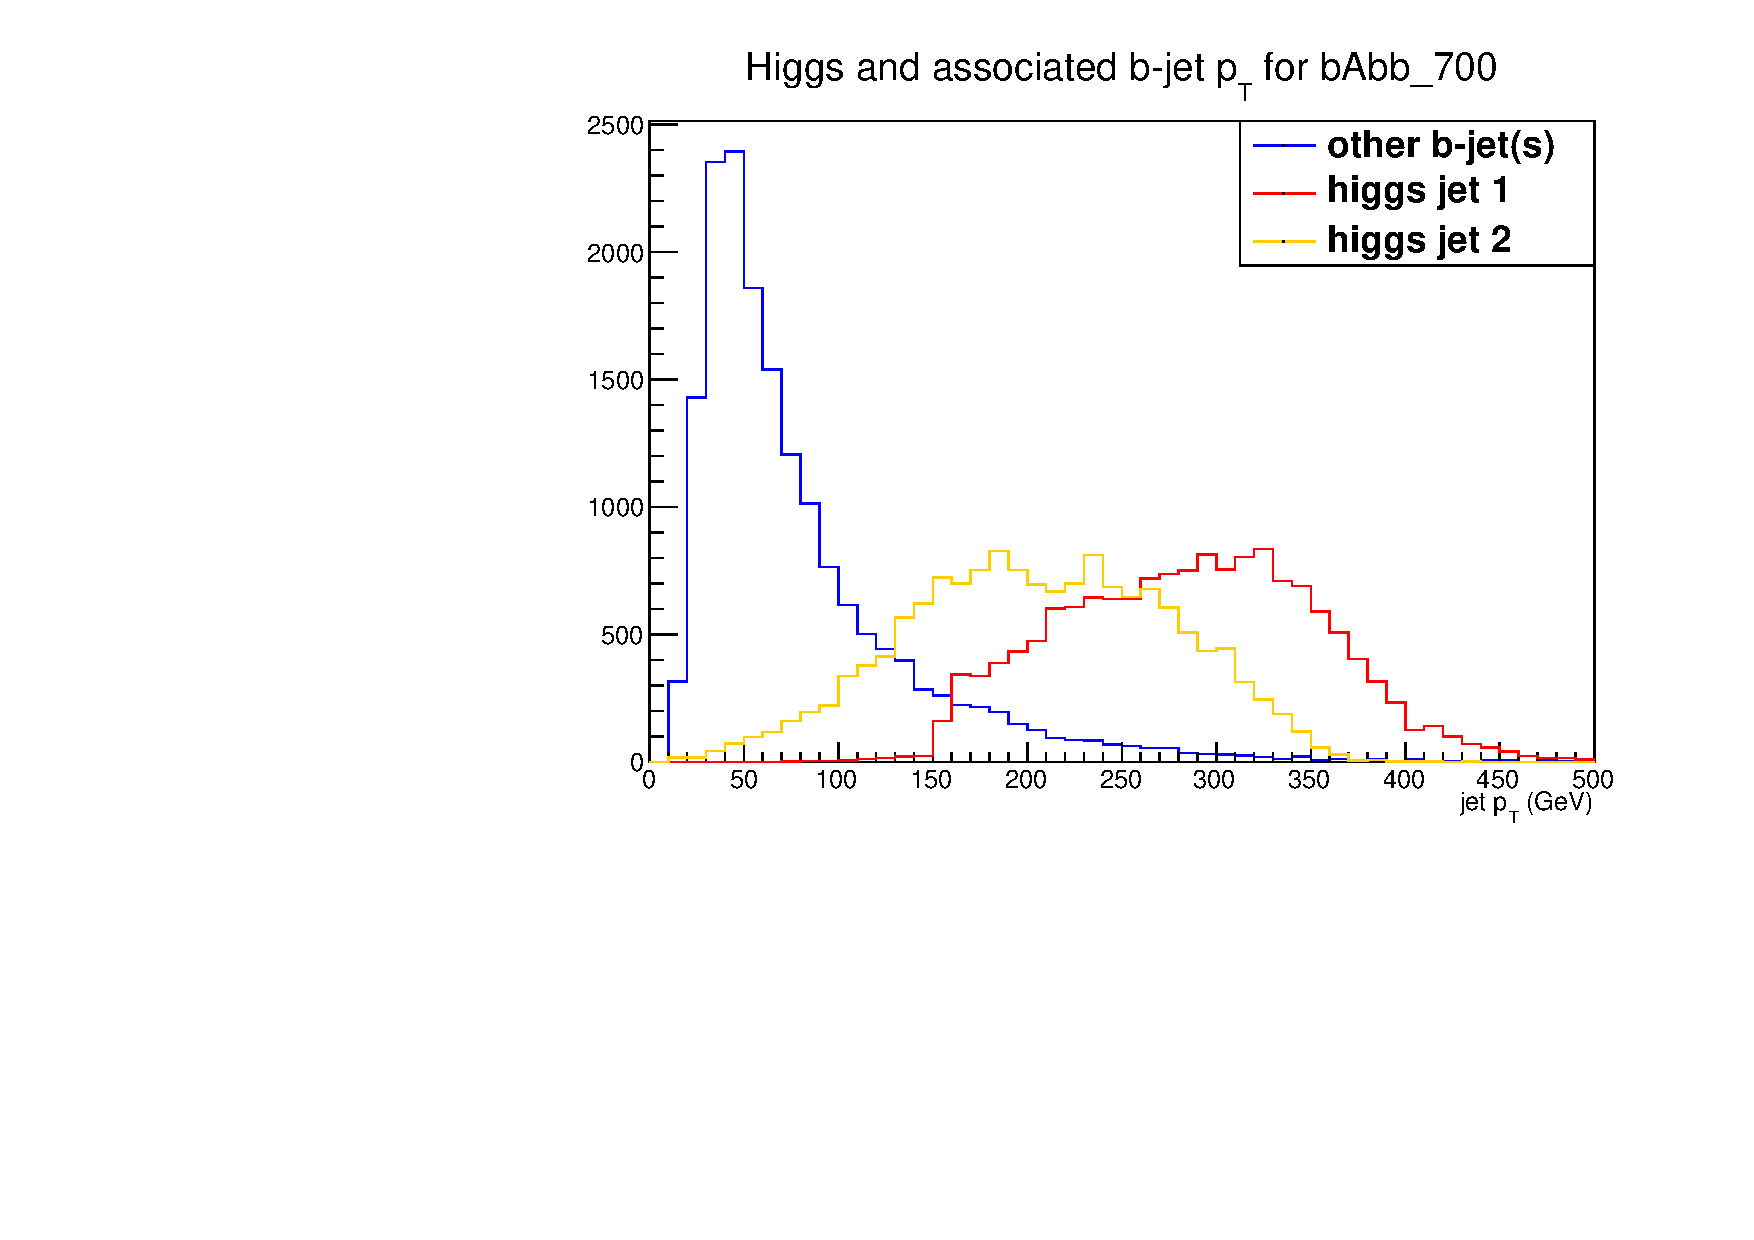
\includegraphics[width=0.33\textwidth]{/Users/caitlinmalone/Documents/Thesis/SignalKin/jet_pt_compare_bAbb_700.pdf}
    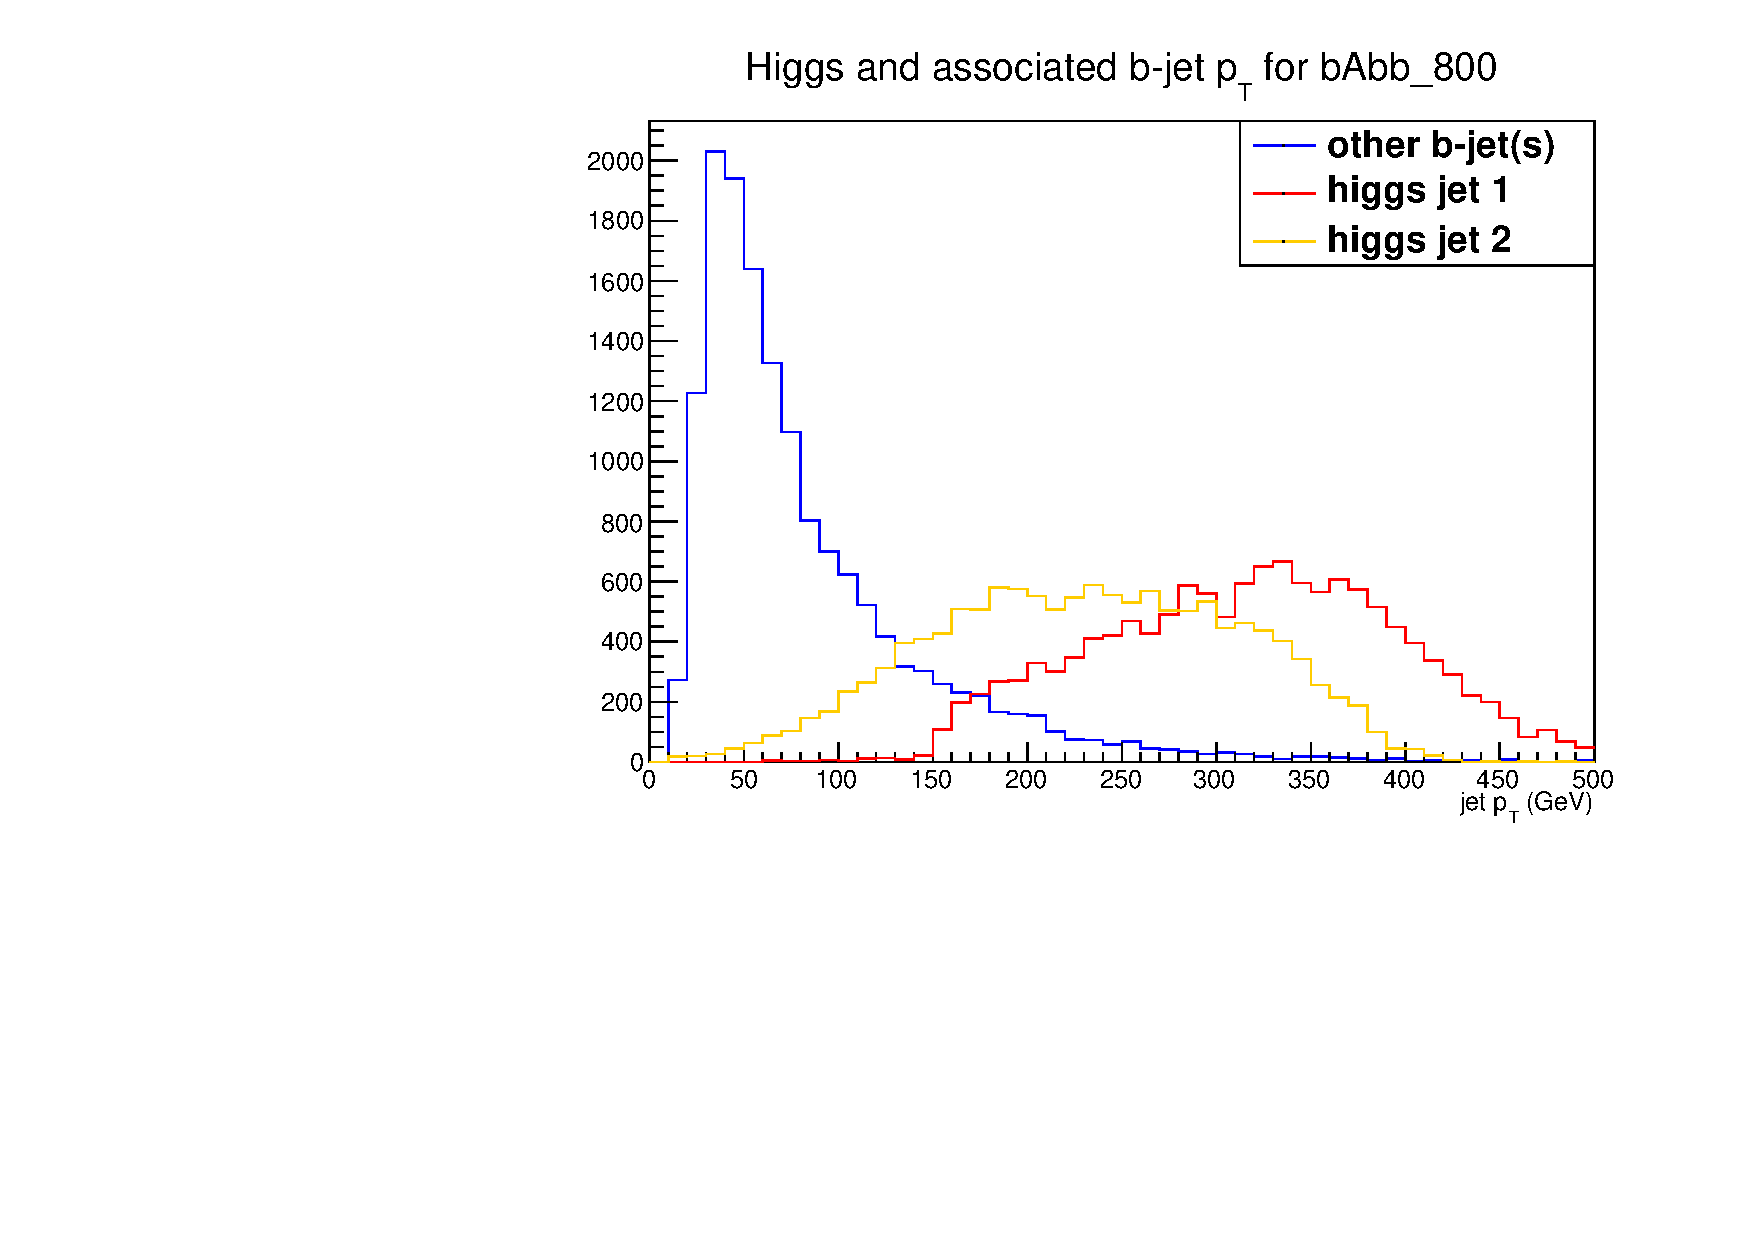
\includegraphics[width=0.33\textwidth]{/Users/caitlinmalone/Documents/Thesis/SignalKin/jet_pt_compare_bAbb_800.pdf}
    \label{fig:pt_higgs_and_associated_jets}
    \caption{The \pt of the two jets from the Higgs (classified as ``first'' and ``second'' based
    on which one has more \pt in the event), and all other $b$-tagged jet(s) in the event.
    The peaks at about 155 GeV and 55 GeV is a result of the trigger turn-on points and
    associated cut(s).  }
\end{figure}
%----------------------------------------------





\subsection{Validation of Qualitative Shape Differences}
\subsection{Jet Modifications}
\subsection{Topology-Based Energy Recovery Algorithm}
\subsection{\pt-Based Energy Recovery Algorithm}
 

